\documentclass[a4paper]{article}

\renewcommand{\contentsname}{Obsah} %rename ToC to Obsah
\renewcommand{\refname}{Literatura} %rename Bibliography to Literatura

%--------packages
\usepackage{graphicx} % images
\graphicspath{figures/}
\usepackage[hidelinks]{hyperref} %clickable links with no ugly box
\usepackage{amsmath}
\usepackage{amsfonts}
\usepackage{mathtools}
\usepackage[czech]{babel} %čeština

%
% \linespread{1.5}

\title{Barevné polarizační zobrazování pro bioaplikace \\rešerše}
\author{Prokop Beneš}
\date{Prosinec 2024}

\numberwithin{equation}{section}

\begin{document}
	\maketitle
	\newpage

	\tableofcontents
	\newpage

    \section{Úvod}
    Barevné polarizační zobrazování představuje inovativní přístup k analýze optických vlastností materiálů,
    který se stále více prosazuje v mnoha oborech a to i v medicínských tak i biologických aplikacích.\cite{biomedical,spie} Využití polarizace světla umožňuje získávat informace o strukturálních a povrchových vlastnostech vzorků, které jsou běžnými metodami prakticky nedostupné. \cite{photonics}
    \par Tato práce si klade za cíl teoreticky zpracovat problematiku barevného polarizačního zobrazování zpohledu fyziky a prozkoumat jeho možnosti v biologických aplikacích, zejména při studiu rostlinných vzorků.V této práci bude využita polarizační kamera BFS-U3-51S5PC-C s integrovaným senzorem Sony IMX250MYR,přičemž se zaměříme na její schopnost snímat a kombinovat polarizační a barevná obrazová data. \cite{flir,teledyne,senzor}
	\newpage
        
	\section{Polarizace}
    Elektromagnetické vlny mají velmi široký spektrální interval. My budeme uvažo-
    \\vat elektromagnetické vlnění pro nás viditelné. Tento interval elektromagnetického vlnění se nachází v intervalu přibližně 380 - 720nm. O elektromagnetickém vlnění v tomto intervalu budeme mluvit jako o světle. \cite{maly}
    \par Elektromagnetická postupná vlna je vlna příčná, což znamená, že elektrické a magnetické pole jsou kolmé na směr šíření. To znamená, že existuje dva nezávislé směry pro vektory těchto polí, mluvíme o dvou nezávislých My se zaměříme na popis elektrické složky vlny $\vec{E}$, protože vektor magnetické složky $\vec{B}$ je určena vztahem $\vec{B}= \frac{1}{v}\vec{s}\times\vec{E}$, kde $\vec{s}$ je vektor udávající směr šíření. Když zvolíme souřadný systém tak, že směr šíření je $\vec{s}=z$. Pak můžeme jako bázi příčné roviny, ve které se nachází $\vec{E}$, použít osy $x$ a $y$. Obecný vektor elektrického pole pak lze rozložit na složky směřující podél souřadných os.


    %dooznačit všechny proměnné!!!!!!!!!!!!!!!!!!!!!!!!!!!!!
    \begin{equation} \label{eq:1}
        \vec{E} = E_x\vec{x} + E_y\vec{y}
    \end{equation}
    Pokud budeme uvažovat harmonické postupné vlny, můžeme díky principu superpozice zvolit vlnu s různou amplitudou a s různým fázovým posunem:
    \begin{equation} \label{eq:2}
        \vec{E}(\vec{r},t) = E_{x0} e^{i(\omega t - kz + \varphi_1)} \vec{x} + 
                             E_{y0} e^{i(\omega t - kz + \varphi_2)} \vec{y}
    \end{equation}
    \par Fázový rozdíl těchto dvou složek můžeme vyjádřit jako 
    \begin{equation} \label{eq:3}
        \delta \varphi = (\omega t -kz + \varphi_1) - (\omega t -kz + \varphi_2) = \varphi_1 - \varphi_2
    \end{equation}
    ten nezávisí ani na čase ani na poloze v prostoru. Zvolíme si libovolné místo v prostoru jako $z = z_0$, můžeme sledovat časový průběh elektrického pole $\vec{E}(t) = \vec{E}(z_0,t)$
    \begin{equation} \label{eq:4}
        \vec{E}(t) = E_{x0} \vec{x} e^{i(\omega t + \varphi_1')} + E_{y0} \vec{y} e^{i(\omega t + \varphi_2')}
    \end{equation}
    kde $\varphi_i' = \varphi - kz_0$. Znovu tedy platí to samé pro rozdíl fází
    \begin{equation} \label{eq:5}
        \delta \varphi = \varphi_1 - \varphi_2 = \varphi_1' - \varphi_2' = (\varphi_1 - kz_0) - (\varphi_2 - kz_0)
    \end{equation}
    \par Z toho tedy vyplývá, že pro fázový rozdíl není důležité, ve kterém místě budeme průběh elektrického pole sledovat. Není třeba se zaobírat konrétními hodnotami fází, rozlišujeme pouze jejich rozdíl $\delta \varphi$.Reálná část rovnice (\ref{eq:4}) má tvar:
    \begin{equation} \label{eq:6}
        \vec{E}(t) = E_{x0}\vec{x}\cos(\omega t + \varphi_1) + E_{y0}\vec{y}\cos(\omega t + \varphi_2)
    \end{equation}
    je parametrickou rovnicí elipsy. Vektor elektrického pole $\vec{E}$ tedy v daném místě opisuje křivku, která má tvar elipsy. Tato elektromagnetická vlna je tedy elipticky polarizovaná. 
    \par Vlny tvaru (\ref{eq:4}), můžeme psát pomocí komplexního vektoru o dvou složkách $\hat{\vec{E}} \in \mathbb{C}^2$, 
    \begin{equation}
        \vec{E}(z,t) = \big(E_{x0} e^{i\varphi_1} \vec{x} + E_{y0} e^{i\varphi_2} \vec{y} \big)  e^{i(\omega t - kz)} = \hat{\vec{E}} e^{i(\omega t-kz)}
    \end{equation}
    \begin{equation}
        \hat{\vec{E}} = \begin{pmatrix} \hat{E}_1 \\ \hat{E}_2 \end{pmatrix} = \begin{pmatrix} E_{x0} \, e^{i \varphi_1} \\ E_{y0} \, e^{i \varphi_2} \end{pmatrix}	 \in \mathbb{C}^2
    \end{equation}
    \par Jeden pro nás velmi důležitý speciální případ je vlna, která je lineárně polarizovaná. Ta nastává, pokud vektor elektrické intenzity $\vec{E}$ kmitá jednom daném směru. 
    \par Tento případ nastává pro fázový posun $\delta \varphi \in \{0,\pi\}$, což pak můžeme zapsat jako
    \begin{equation} \label{eq:7}
        \vec{E} = E_0 \vec{n} e^{i(\omega t + \varphi]}
    \end{equation}
    neboli 
    \begin{equation} 
        \hat{\vec{E}} = E_0 \, \vec{n} \, e^{i\varphi} = E_0 \begin{pmatrix} \cos \theta \\ \sin \theta \end{pmatrix} e^{i\varphi}
    \end{equation}
    kde jednotkový vektor $\vec{n} = (n_x,n_y) = (\cos \theta, \sin \theta)$ znázorňuje směr kmitání elektrického pole $\vec{E}(t)$ v rovině $xy$ a úhel $\theta$ značí odklon tohoto vektoru od osy $x$. \cite{schmidt}
    \par Jedním z nejobvyklejších způsobů kde se v životě potkáme s polarizovaným světlem je bězná polarizace odrazem. Tento proces vychází ze Snellova zákona následujícím způsobem: 
    \begin{equation}
        n_1 \sin \theta_i = n_2 \sin \theta_t
    \end{equation}
    je Snellův zákon a $n_1$ a $n_2$ značí index lomu daného prostředí v kterém se světlo šíří.  $\theta_i$ je úhel dopadu, $\theta_t$ je úhel lomu. Úhlu pod kterým musí světlo dopadnout aby bylo lineárně polarizováno se říká úhel Brewsterův. 
    \begin{figure}[ht]
        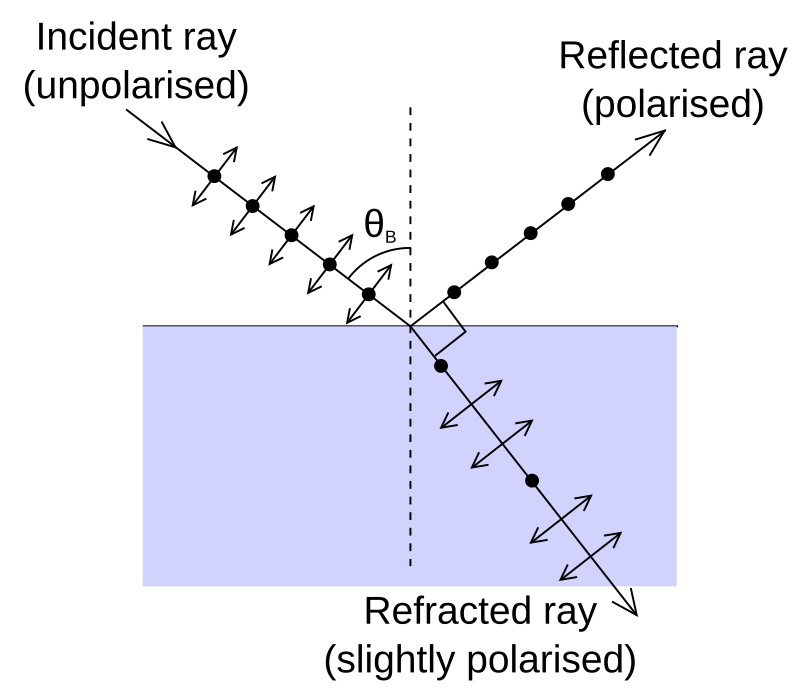
\includegraphics[width=7cm]{figures/Brewster.png}
        \centering
    \end{figure}
    \par Pro něj platí že $\theta_i + \theta_t = 90^{\circ}$, tedy, že úhel dopadajícího, tedy i odraženého světla musí svírat se světlem lomeným úhel devadesáti stupňů. Tedy $\theta_t = 90^{\circ} - \theta_i$ dosadíme do Snellova zákona. 
    \begin{equation}
        \!
        \begin{aligned}
            n_1 \sin \theta_i &= n_2 \sin (90^{\circ} - \theta_i) \\
            n_1 \sin \theta_i &= n_2 \cos \theta_i
        \end{aligned}
    \end{equation} 
    což nám po úpravě dá 
    \begin{equation}
        \frac{n_2}{n_1} = \frac{\sin \theta_i}{\cos \theta_i}
    \end{equation}
    neboli
    \begin{equation}
        \tan \theta_i = \frac{n_2}{n_1}
    \end{equation}
    Kde námi požadovaný Brewsterův úhel dostaneme jako
    \begin{equation}
        \theta_B = \arctan \frac{n_2}{n_1}
    \end{equation}
    Nepolarizované světlo dopadjící pod tímto úhlem se od rozhraní odráží pouze se složkou kolmou k rovině rozhraní. \cite{hecht} 
    \\Takto lineárně polarizované světlo pro nás bude v následujícím textu velmi důležité. Na princip lineárně polarizovaného světla totiž stojí princip naší barevné polarizované kamery BFS-U3-51S5PC-C

    \newpage
	\section{Aplikace Polarizace}
	Senzor kamery s kterou pracujeme má na svém senzoru mikrostrukturu, která se chová jako polarizátor přicházejícího světla, jelikož je jeho rozměr dostatečně malý na to, aby jím prošla jen určitá složka světla v daném úhlu podle úhlu samotného polarizátoru. Senzor samotný má každý pixel sestaven ze čtyř podpixelů kde každý z nich má přes sebe jiný úhel polarizátoru a to $90^{\circ}, 45^{\circ}, 135^{\circ}, 0^{\circ}$ podle směru hodinových ručiček začínaje vlevo v rohu.
    \begin{figure}[h]
        \includegraphics[width=8cm]{figures/senzor.jpg}
        \centering
    \end{figure}

    \subsection{Senzor Sony IMX250MYR}
    Kamera BFS-U3-51S5PC-C se senzorem Sony IMX250MYR, se kterou pracujeme, se již objevuje ve výzkumných publikacích využívajících polarizované snímání. Ať už z pohledu kalibrace samotného senzoru, nebo se také řeší demosaicing snímků získaných z tohoto senzoru, samozřejmě jsou publikovány i výzkumné články zkoumající chování polarizace za pomocí tohoto senzoru.\cite{kalibrace,kalibrace2,demosaicing,aplikace} Z kamery lze dostat snímky díky poskytnutému softwaru. Zde si můžeme nastavit například white balance, expozici, kontrast nebo třeba gamma korekci. Získáme ze software kamery RAW fotku, kterou jsmě schopni zpracovat například v MATLABu s tím, že je potřeba foktu z RAW formátu upravit do formátu pro nás vhodného pro nějakopu další analýzu. Na to máme připravený krátký skript v MATLABu, nejprve je třeba si udělat demosaicing pomocí inbuilt matlab funkce "demosaic", která nám vrátí RGB snímek dekódovaný podle specifikovaného uspořádání Bayerovského filtru, který je v tomto případě RGGB. \cite{matlab} Pokud chceme z kamery dostat celkový snímek je třeba tento demosaicovaný snímek po blocích zprůměrovat. Dále pokud budeme chtít snímky obsahující informace o polarizaci dané fotky tak je třeba si takovýto obrázek rozdělit na čtyři snímky s úhly polarizace podle toho z jaké části superpixelu si je vezmeme. Výsledkem tedy budou čtyři fotky, které obsahují pouze informace z těch daných úhlů samotných pixelů. Z těch jsme poté, pomocí například Stokesových parametrů, určit Degree of Linear Polarization (DoLP) a nebo Angle of Linear Polarization (AoLP). Tyto parametry nám mohou poskytnout důležité informace lidským okem  nepozorovatelné. \cite{aolp}

    \subsection{Využití polarizace ve výzkumu}
    Specifických využití polarizačního zobrazování je veliké množství a proto si ukážeme jen některé obecné zajímavé aplikace, včetně možným aplikacím v oblasti biologie a biomedicíny. Možností použití polarizačního barevného senzoru, je díky jeho schopnosti snímat i polarizované barevmé snímky, velmi zajímavé. Pomocí polarizace jsem schopni ze snímků dostat informace, které by bylo za použití konvenčních metod snímání velmi náročné. To ať už kvůli odrazivosti materiálů materiálů které snímáme, nebo světelných podmínek za kterých snímáme. Takovou aplikací může být například výrobní linka léků. Normální snímání samotných balení s léky může být náročné, když se jedná o prášky bílé na hliníkové fólii. Pak nám na rozpoznávání naplňěnosti balení, které chceme snímat kamerou, usnadní polarizační senzor. Díky rozdílu DoLP výrazně jednodušeji rozpoznáme zda v daném místě balení léků jeden chybí nebo ne. \cite{pharmaceutics}
    \par Dalším možným využitím polarizačního zobrazování je při zkoumání průhle-
    \\dných materiálů. Při zkoumání průhledných materiálů a objektů nám toho opět standardní senzory hodně neřeknou. Zato polarizační zobrazování nám poskytne díky AoLP nebo DoLP spoustu informací okem také nepozorovatelných. Například vnitřní napětí takovýchto objektů je bez polarizace nepozorovatelné, ale díky AoLP jsme jej schopni pozorovat i měřit. \cite{stresy}
    \par Další zajímavé využití polarizačního snímání bude měření koncentrací různých roztoků, například vodných roztoků cukrů. Jelikož je cukr chirální, tedy prostorově asymetrický, mění tedy optické vlastnosti roztoku a tedy i světla jím procházejícím. \cite{chiralita} Tyto změny jsme díky změně v polarizaci schopni pozorovat polarizační kamerou. K takovému měření budeme potřebovat Stokesovy parametry ze kterých si jsme schopni vypočítat AoLP. Úhel lineární polarizace nám právě o koncentraci roztoku poví co nás zajímá. Zobrazení tohoto úhlu polarizace je důležité, protože jsme díky němu schopni porovnat proti sobě různé koncentrace cukernatých roztoků, které bychom bez polarizační kamery nezjistili. \cite{sugar}

    \newpage
    \addcontentsline{toc}{section}{Literatura}
    \begin{thebibliography}{99}
        \bibitem{biomedical} \textit{Optical Polarization in Biomedical Applications} \url{https://link.springer.com/book/10.1007/978-3-540-45321-5}
        \bibitem{spie} \textit{Polarized light imaging in biomedicine: emerging Mueller matrix methodologies for bulk tissue assessment} \url{https://www.spiedigitallibrary.org/journals/journal-of-biomedical-optics/volume-20/issue-6/061104/Polarized-light-imaging-in-biomedicine--emerging-Mueller-matrix-methodologies/10.1117/1.JBO.20.6.061104.full}
        \bibitem{photonics} \textit{Polarization-Based Imaging: Basics and Benefits} \url{https://www.photonics.com/Articles/Polarization-Based_Imaging_Basics_and_Benefits/a60734}
        \bibitem{flir} \url{https://www.flir.eu/globalassets/support/iis/knowledge-base/getting-started-with-bfs-polarized-cameras.pdf}
        \bibitem{teledyne} \url{https://www.teledynevisionsolutions.com/learn/learning-center/machine-vision/imaging-reflective-surfaces-sonys-first-polarized-sensor/}
        \bibitem{senzor} \url{https://www.sony-semicon.com/files/62/flyer_industry/IMX250_264_253MZR_MYR_Flyer_en.pdf}
        \bibitem{maly} Malý P., \textit{Optika}, Nakladatelství Karolinum, 2008
        \bibitem{schmidt} Schmidt J., \textit{Vlnění, optika a atomová fyzika}, \url{https://physics.fjfi.cvut.cz/~schmijos/voaf/skriptaVOAF.pdf}
        \bibitem{hecht} Hecht E., \textit{Optics}, 4th Ed, Pearson, 2002
        \bibitem{kalibrace} \url{https://opg.optica.org/ao/fulltext.cfm?uri=ao-61-6-C37&id=462441}
        \bibitem{kalibrace2} \url{https://ieeexplore.ieee.org/document/9834097}
        \bibitem{demosaicing} \url{https://www.mathworks.com/matlabcentral/fileexchange/131763-demosaicing-algorithm-for-sony-imx250myr}
        \bibitem{aplikace} \url{https://ieeexplore.ieee.org/stamp/stamp.jsp?tp=&arnumber=9639607}
        \bibitem{matlab} \url{https://www.mathworks.com/help/images/ref/demosaic.html}
        \bibitem{aolp} \url{https://www.sony-semicon.com/en/technology/industry/polarsens.html}
        \bibitem{pharmaceutics} \url{https://www.sony-semicon.com/en/technology/industry/polarsens.html}
        \bibitem{stresy} \url{https://thinklucid.com/tech-briefs/polarization-explained-sony-polarized-sensor/}
        \bibitem{chiralita} \url{https://www.biorxiv.org/content/10.1101/2020.08.16.252718v1.full.pdf}
        \bibitem{sugar} \url{https://thinklucid.com/polarized-camera-resource-center/evaluating-sugar-concentration-in-water/}
    \end{thebibliography}
\end{document}